\chapter{Neural Networks and Deep Learning}

\section{Introduction to Deep Learning}
机器学习本质上就是训练模型来完成\textbf{从输入到输出($\bm{X\to Y}$)的映射}。例如, 给定一张猫的照片, 机器学习模型可以输出``这是一只猫''的结论。

\vspace{0.5\baselineskip} % 半行距

深度学习有3大要点:
\begin{itemize}	
	\item Data
	\item Computation
	\item Algorithms
\end{itemize}

Data可以分为Structured Data和Unstructured Data。Structured Data是指有固定格式的数据, 例如表格、数据库等。Unstructured Data是指没有固定格式的数据, 例如图片、音频、视频等。

Computation是指计算机的计算能力, 例如CPU、GPU、TPU等。

Algorithms是指算法, 例如Logistic Regression、SVM、Neural Networks等。

\section{Neural Networks Basics}

\subsection{Binary Classification}

表 \ref{tab:notations} 是本章用到的符号说明。

\begin{table}[h]
	\centering
	\begin{threeparttable}
	%%%%%
	\caption{Notations}
	%
	\begin{tabular}{clcc}
		\hline
									& \textbf{Notation}                         & \textbf{Description} & \textbf{Meaning}                                                   \\ \hline
		\multirow{5}{*}{Sizes}      & $m$                                       & value                & 样本容量                                                               \\
									& $n_x$                                     & value                & 单个样本的特征数(输入)                                                \\
									& $n_y$                                     & value                & 单个样本的标签数(输出)                                                \\
									& $n_h^{[l]}$                               &                      &                                                                    \\
									& $L$                                       &                      &                                                                    \\ \hline
		\multirow{9}{*}{Objects}    & $x^{(i)} \in \mathbb{R}^{n_x}$            & vector               & 第$i$个样本数据                                                          \\
									& $X \in {\mathbb{R}^{n_x \times m}}$       & matrix               & 输入矩阵                                                               \\
									& $a^{(i)} / y^{(i)} \in \mathbb{R}^{n_y}$  & vector               & 第$i$个样本的标签                                                         \\
									& $Y \in {\mathbb{R}^{n_y \times m}}$       & matrix               & 标签矩阵($n_y=1$时退化为行向量$y$)                                    \\									
									& $\hat{y}^{(i)} \in \mathbb{R}^{n_y}$      & vector               & 第$i$个样本的标签预测值向量                                                \\
									& $\hat{Y} \in {\mathbb{R}^{n_y \times m}}$ & matrix               & 标签预测值矩阵($n_y=1$时退化为行向量$\hat{y}$)   						\\
									& $W \in \mathbb{R}^{n_x \times n_y}$       & matrix               & 权重矩阵($n_y=1$时退化为列向量$w$)                                    \\
									& $b \in \mathbb{R}^{n_y}$                  & vector               & 标签偏置值向量                                                        \\
									& $W^{[l]}$                                 &                      &                                                                    \\
									& $b^{[l]}$                                 &                      &                                                                    \\ \hline
		\multirow{2}{*}{Other}      & $J(x,W,b,y)$ or $J(\hat{y},y)$            & function             & 代价函数                                                               \\
									& $\mathrm{d}\mathrm{var}$                  & differential         & 代价函数对变量$\mathrm{var}$的微分,即${\mathrm{d}J}/{\mathrm{d}\mathrm{var}}$ \\ \hline
	\end{tabular}
	%
	\label{tab:notations} %%%
	\begin{tablenotes}
		\item[*] 通常情况下$(i)$表示第$i$个样本,而$[l]$表示第$l$层。
	\end{tablenotes}
	%%%%%
	\end{threeparttable}
\end{table}

\subsection{Logistic Regression}

对于\textbf{二元分类模型,$\bm{n_y=1}$},相关公式如下:
\begin{equation}
	\hat{y}^{(i)} = \sigma(w^\mathrm{T} x^{(i)} + b) \label{eq:logistic}
\end{equation}
其中sigmoid函数$\sigma(z)$定义为:
\begin{equation}
	\sigma(z) = \frac{1}{1 + \mathrm{e}^{-z}} \label{eq:sigmoid}
\end{equation}
该函数可以把实数域$\mathbb{R}$映射到区间$(0, 1)$,如图 \ref{fig:sigmoid} 所示。而$z = w^\mathrm{T} x + b$为线性函数,$w$为权重(weight),$b$为偏置(bias)。
\begin{figure}[h]
	\centering
	\includesvg[width=8cm]{sigmoid}
	\caption{Sigmoid 函数,关于点(0, 0.5)对称}
	\label{fig:sigmoid}
\end{figure}

\vspace{0.5\baselineskip}
对某一个样本而言,Loss function(误差函数)定义为:
\begin{equation}
	L(\hat{y}^{(i)}, y^{(i)}) = -\left[y^{(i)} \log \hat{y}^{(i)} + (1 - y^{(i)}) \log (1 - \hat{y}^{(i)})\right] \label{eq:loss}
\end{equation}
该函数与方差类似,当样本的误差越大,Loss function的值越大,如图 \ref{fig:loss} 所示。
\begin{figure}[h]
	\centering
	\includesvg[width=8cm]{LossFunction}
	\caption{Loss Function 误差函数}
	\label{fig:loss}
\end{figure}

对整个模型而言,Cost function(代价函数)定义为:
\begin{equation}
	J(w, b) = \frac{1}{m} \sum_{i=1}^{m} L(\hat{y}^{(i)}, y^{(i)}) = -\frac{1}{m} \sum_{i=1}^{m} \left[y^{(i)} \log \hat{y}^{(i)} + (1 - y^{(i)}) \log (1 - \hat{y}^{(i)})\right] \label{eq:cost}
\end{equation}
相当于误差函数的平均值。

\subsection{Gradient Descent}

训练过程使用\textbf{梯度下降(Gradient Descent)算法},即:
\begin{equation}
	\mathrm{var} = \mathrm{var} - \alpha \frac{\mathrm{d}J}{\mathrm{d}\mathrm{var}} \label{eq:gradient}
\end{equation}

其中$\mathrm{var}$为一个需要调整的参数,$\alpha$为学习率(Learning Rate)。对于Logistic Regression,梯度下降算法的表达式为:
\begin{equation}
	\begin{aligned}
	w &:= w - \alpha \frac{\mathrm{d}J}{\mathrm{d}w} \\
	b &:= b - \alpha \frac{\mathrm{d}J}{\mathrm{d}b}
	\end{aligned} 
	\label{eq:gradient_logistic}
\end{equation}
其中$:=$表示赋值,通过不断更新$w$, $b$的值使$J$尽可能小。下面介绍具体实现

\vspace{0.5\baselineskip}
对于一个样本,有
\begin{equation}
	\begin{aligned}
	z &= w^\mathrm{T} x^{(i)} + b \\
	\hat{y}^{(i)} &= \sigma(z) \\
	L(\hat{y}^{(i)}, y^{(i)}) &= -\left[y^{(i)} \log \hat{y}^{(i)} + (1 - y^{(i)}) \log (1 - \hat{y}^{(i)})\right]
	\end{aligned} 
	\label{eq:gradient_logistic_sample}
\end{equation}
进行求导($x$, $y$均为常量),有
\begin{equation}
	\begin{aligned}
	&\frac{\mathrm{d}L}{\mathrm{d}\hat{y}^{(i)}} = -\frac{y^{(i)}}{\hat{y}^{(i)}} + \frac{1 - y^{(i)}}{1 - \hat{y}^{(i)}} \\
	&\frac{\mathrm{d}\hat{y}^{(i)}}{\mathrm{d}z} = \frac{\mathrm{e}^{-z}}{(1 + \mathrm{e}^{-z})^2} = \frac{1}{1 + \mathrm{e}^{-z}}(1 - \frac{1}{1 + \mathrm{e}^{-z}}) = \hat{y}^{(i)}(1 - \hat{y}^{(i)})\\
	\end{aligned}
\end{equation}
用链式法则,有
\begin{equation}
	\frac{\mathrm{d}L}{\mathrm{d}z} = \frac{\mathrm{d}L}{\mathrm{d}\hat{y}^{(i)}} \frac{\mathrm{d}\hat{y}^{(i)}}{\mathrm{d}z} = (-\frac{y^{(i)}}{\hat{y}^{(i)}} + \frac{1 - y^{(i)}}{1 - \hat{y}^{(i)}})\hat{y}^{(i)}(1 - \hat{y}^{(i)}) = \hat{y}^{(i)} - y^{(i)}
\end{equation}
进而有
\begin{equation}
	\begin{aligned}
	\frac{\mathrm{d}L}{\mathrm{d}w_j} &= \frac{\mathrm{d}L}{\mathrm{d}z} \frac{\mathrm{d}z}{\mathrm{d}w_j} = x_j^{(i)} (\hat{y}^{(i)} - y^{(i)}) \quad (1 \leqslant j \leqslant n_x) \\
	\frac{\mathrm{d}L}{\mathrm{d}b} &= \frac{\mathrm{d}L}{\mathrm{d}z} \frac{\mathrm{d}z}{\mathrm{d}b} = \hat{y}^{(i)} - y^{(i)}
	\end{aligned}
\end{equation}

\vspace{0.5\baselineskip}
对于整个训练集,在一个循环中我们对每一个样本都进行一次梯度下降,并对所有样本的梯度进行平均,有
\begin{equation}
	\begin{aligned}
		\frac{\mathrm{d}J}{\mathrm{d}w_j} &= \frac{1}{m} \sum_{i=1}^{m} \frac{\mathrm{d}L}{\mathrm{d}w_j} = \frac{1}{m} \sum_{i=1}^{m} x_j^{(i)} (\hat{y}^{(i)} - y^{(i)}) \quad (1 \leqslant j \leqslant n_x)\\
		\frac{\mathrm{d}J}{\mathrm{d}b} &= \frac{1}{m} \sum_{i=1}^{m} \frac{\mathrm{d}L}{\mathrm{d}b} = \frac{1}{m} \sum_{i=1}^{m} (\hat{y}^{(i)} - y^{(i)})
	\end{aligned}
\end{equation}
得到梯度的平均值后,再进行参数更新,即
\begin{equation}
	\begin{aligned}
	w_j &:= w_j - \alpha \frac{\mathrm{d}J}{\mathrm{d}w} \quad (1 \leqslant j \leqslant n_x) \\
	b &:= b - \alpha \frac{\mathrm{d}J}{\mathrm{d}b}
	\end{aligned} 
\end{equation}
这样就完成了一轮梯度下降的循环。重复多次梯度下降,直到$J$收敛或达到最大迭代次数,就得到了最终的$w$, $b$。

\subsection{Vectorization}

一个重要的原则是,在训练过程中要避免使用循环,而是使用向量化的方法。向量化可以调用并行计算,相对于循环的串行计算效率更高。\\
要完成下面的矩阵操作,
\begin{equation}
	Z =
	\begin{bmatrix}
		z^{(1)} & z^{(2)} & \cdots & z^{(m)}
	\end{bmatrix}
	= w^\mathrm{T} X + 
	\begin{bmatrix}
		b & b & \cdots & b
	\end{bmatrix}
\end{equation}
可以使用下面的代码
\begin{python}
import numpy as np
# define X, Y, w, b
Z = np.dot(w.T, X) + b
\end{python}
同理,要实现
\begin{equation}
	\begin{aligned}
		\frac{\mathrm{d}J}{\mathrm{d}w_j} &= \frac{1}{m} \sum_{i=1}^{m} \frac{\mathrm{d}L}{\mathrm{d}w_j} = \frac{1}{m} \sum_{i=1}^{m} x_j^{(i)} (\hat{y}^{(i)} - y^{(i)}) \quad (1 \leqslant j \leqslant n_x)\\
		\frac{\mathrm{d}J}{\mathrm{d}b} &= \frac{1}{m} \sum_{i=1}^{m} \frac{\mathrm{d}L}{\mathrm{d}b} = \frac{1}{m} \sum_{i=1}^{m} (\hat{y}^{(i)} - y^{(i)})
	\end{aligned}
\end{equation}
可以继续使用下面的代码
\begin{python}
def sigmoid(x):
    s = 1 / (1 + np.exp(-x))
    return s


A = sigmoid(Z)
dZ = A - Y
dw = np.dot(X, dZ.T) / m
# sum along the column
db = np.sum(dZ, axis=1) / m
# sum will get a row vector regardless of the axis parameter, so we need to reshape it
db = db.reshape(ny, 1)
\end{python}
\verb|np.sum()| 函数的 \verb|axis| 参数表示沿着哪个维度进行求和,\verb|axis=0| 表示沿着列求和,\verb|axis=1| 表示沿着行求和。

\vspace{0.5\baselineskip}
在 \verb|numpy| 中,矩阵的维度扩充与 \verb|matlab| 类似,可以自动扩充,也可以使用 \verb|reshape| 函数进行扩充。

矩阵(或向量)在保存时,使用了两重方括号,例如 \verb|[[1, 2], [3, 4]] / [[3, 6, 9]]|,而数组仅有一重方括号,例如 \verb|[1, 2, 3, 4]|。
要把数组转换为向量,可以使用 \verb|reshape()| 函数,例如
\begin{python}
A = np.array([1, 2, 3, 4])
print(A)
print(A.shape)
print(A.T)
A = A.reshape(1, 4)
print(A)
print(A.shape)
print(A.T)
\end{python}
输出结果为
\begin{python}
# array, rank=1
[1 2 3 4]
(4,) 
[1 2 3 4]
# vector
[[1 2 3 4]]
(1, 4) 
[[1]
 [2]
 [3]
 [4]]
\end{python}
\verb|reshape()| 是一个$O(1)$的操作,不会影响程序的运行效率。在本课程中不要使用 \verb|rank 1 array|,因为它的维度不是$(n, 1)$或$(1, n)$,在进行矩阵运算时会出现错误。

\vspace{0.5\baselineskip}
为了确保矩阵的维度正确,可以使用 \verb|assert()| 函数,例如
\begin{python}
assert(A.shape == (1, 4))
\end{python}
如果 \verb|A.shape| 不等于 \verb|(1, 4)|,则会报错。

\subsection{Explanation of logistic regression cost function}

对于二元分类模型,我们期望$\hat{y}$尽可能接近$y$,即${y}^{(i)}$等于$1$时,$\hat{y}^{(i)}$接近$1$,而${y}^{(i)}$等于$0$时,$\hat{y}^{(i)}$接近$0$。

当$y^{(i)}=1$时,得到正确分类的概率为$\hat{y}^{(i)}$;而当$y^{(i)}=0$时,得到正确分类的概率为$1-\hat{y}^{(i)}$。因此,对于第$i$个样本,可以使用下面的公式来表示这个概率:
\begin{equation}
	P(y^{(i)} | x^{(i)}; w, b) = (\hat{y}^{(i)})^{y^{(i)}} (1-\hat{y}^{(i)})^{1-y^{(i)}}
\end{equation}
假如各个样本是独立的,那么所有样本得到正确分类的概率为
\begin{equation}
	\begin{aligned}
		P(y | x; w, b) &= \prod_{i=1}^{m} P(y^{(i)} | x^{(i)}; w, b)\\
		&= \prod_{i=1}^{m} (\hat{y}^{(i)})^{y^{(i)}} (1-\hat{y}^{(i)})^{1-y^{(i)}}
	\end{aligned}
\end{equation}
为了避免使用指数运算,可以在等式两边取对数,得到
\begin{equation}
	\begin{aligned}
		\log P(y | x; w, b) &= \sum_{i=1}^{m} \log (\hat{y}^{(i)})^{y^{(i)}} (1-\hat{y}^{(i)})^{1-y^{(i)}}\\
		&= \sum_{i=1}^{m} \left[ y^{(i)} \log \hat{y}^{(i)} + (1-y^{(i)}) \log (1-\hat{y}^{(i)}) \right]
	\end{aligned}
\end{equation}
习惯上等式右边要取平均值,因此可以得到
\begin{equation}
	\frac{1}{m} \log P(y | x; w, b) = \frac{1}{m} \sum_{i=1}^{m} \left[ y^{(i)} \log \hat{y}^{(i)} + (1-y^{(i)}) \log (1-\hat{y}^{(i)}) \right]
\end{equation}
我们期望这个值越大越好,为了使用梯度下降法,可以对上式取负号,得到
\begin{equation}
	J(w, b) \triangleq - \frac{1}{m} \sum_{i=1}^{m} \left[ y^{(i)} \log \hat{y}^{(i)} + (1-y^{(i)}) \log (1-\hat{y}^{(i)}) \right]
\end{equation}
这就是代价函数的定义。我们期望代价函数的值越小越好,因此可以使用梯度下降法来求解$w$和$b$。

\section{Shallow Neural Networks}
在上一节中,我们构建的模型本质上是一个一层的神经“网络”。在本节中,我们将构建一个两层的神经网络,也就是一个\textbf{浅层神经网络(Shallow Neural Network)}。

\begin{figure}[h]
	\centering
	\begin{tikzpicture}[x=1.5cm, y=1.5cm, >=stealth]
		\def\nx{3}
		\def\nu{4}
		% 输入层
		\foreach \i in {1,...,\nx}
			\node[circle, draw=none] (x\i) at (0,2-\i) {$x_\i^{(i)}$};
		\foreach \i in {1,...,\nx}
			\node[coordinate] (lx\i) at (0.2,2-\i) {};
		
		% 隐藏层
		\foreach \h in {1,...,\nu}
			\node[circle, draw=blue, fill=white, inner sep=0pt, minimum size=10mm] (h\h) at (2,2.5-\h) {$a_\h^{[1](i)}$};
		
		% 输出层
		\node[circle, draw=yellow, fill=white, inner sep=0pt, minimum size=10mm] (o) at (4,0) {$a^{[2](i)}$};
	
		% 预测值
		\node[circle, draw=none] (yhat) at (5.5,0) {$\hat{y}^{(i)}$};
		
	
		% 连接
		\foreach \i in {1,...,\nx}
			\foreach \h in {1,...,\nu}
				\draw[->, color=base1] (lx\i) -- (h\h);
		
		\foreach \h in {1,...,\nu}
			\draw[->, color=base1] (h\h) -- (o);
		
		\draw[->, color=base1] (o) -- (yhat);
		
		% 标签
		\def\labely{-2}
		\draw [decorate,decoration={calligraphic brace,amplitude=4pt,mirror}] (-0.35,\labely) -- (0.35,\labely) node [green,midway,yshift=-0.5cm] {输入层};
		\draw [decorate,decoration={calligraphic brace,amplitude=4pt,mirror}] (1.5,\labely) -- (2.5,\labely) node [blue,midway,yshift=-0.5cm] {隐藏层};
		\draw [decorate,decoration={calligraphic brace,amplitude=4pt,mirror}] (3.5,\labely) -- (4.5,\labely) node [yellow,midway,yshift=-0.5cm] {输出层};
		\draw [decorate,decoration={calligraphic brace,amplitude=4pt,mirror}] (5.15,\labely) -- (5.85,\labely) node [red,midway,yshift=-0.5cm] {预测值};
	
	\end{tikzpicture}
	\caption{Shallow Neural Network 浅层神经网络}
	\label{fig:shallow_nn}
\end{figure}

\begin{figure}[h]
	\centering
	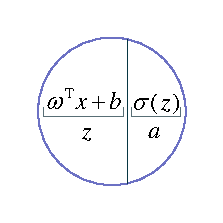
\includegraphics[width=5cm]{node.pdf}
	\caption{单个节点的结构}
	\label{fig:node}
\end{figure}